% !TeX root = ../analysisnote.tex

\section{Analysis setup}

This section describes the setup of analysis. 
The first part of this section introduces STAR Fixed Target(FXT) mode. 
Second one is dataset and event selection used in the analysis. 
Third, badrun rejection and centrality determination are discussed.

%-------------------------------
\subsection{Introduction of FXT}

There are two modes at RHIC-STAR, Fixed Target mode and Collider mode. 
FXT mode of STAR experiment covers center of mass energy($\snn$) from 3 to 13.7 GeV, which extends the measurement to lower energy intervals.
In this way, FXT mode could reach higher baryon density region(up to 750 MeV). 
To achieve this goal, One piece of gold foil would be fixed at the end of Time Projection Chamber(TPC) as target.
And the accelerated gold beam from west would collide with it. Fig.~\ref{fig:FXTmode} shows the schematic plot for fixed target mode.
\begin{figure}[hbt!]
\centering
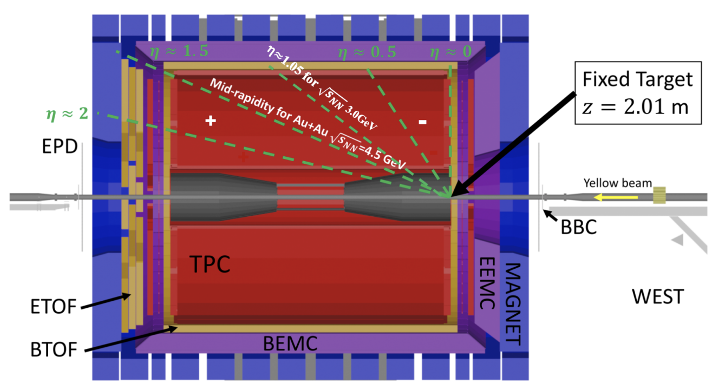
\includegraphics[width=0.85\linewidth]{figures/chapter01/FXTmode.png}
\caption{The setup of Fixed Target mode at STAR.}
\label{fig:FXTmode}
\end{figure}

The laboratory system should be transferred to the center of mass system, 
if one want to analysis physical observation conveniently. 
According to the Lorentz transformation, Rapidity(y) of the final state particle in the Center of Mass System(CMS) could be calculated as equation~\ref{eq:transf_rap}, 
where $y_{lab}$ is rapidity of emitted particle in the laboratory frame, $y_{beam}$ is rapidity of gold beam in the CMS.
And we would discuss flow measurement based in the Center of Mass System.
\begin{equation}
    y_{CMS} = y_{lab} - y_{beam}
\label{eq:transf_rap}
\end{equation}

%-------------------------------
\subsection{Dataset and event selection}

In this analysis, four energies($\snn=3, 3.2, 3.5, 3.9 GeV$) from fixed target mode are involved.
The events from minimum bias trigger are selected. And vertex cut in the X and Y direction applied to exclude the events from beam pipe, 
vertex cut along the Z direction to ensure that selection events are from collision on the gold foil.
The detailed trigger and vertex cut are summarized in the TABLE.~\ref{tab:dataset}
\begin{table}
\caption{Dataset and event cuts for $\snn=3, 3.2, 3.5, 3.9 GeV$.}
\label{tab:dataset}
\begin{tabular}{|c|c|c|}
\hline
nHitsFit$>=$15 \\ \hline
$\chi^{2}_{topo}<10$ \\ \hline
\end{tabular}
\end{table}


%-------------------------------
\subsection{Badrun rejection and centrality determination}
